\chapter{ATRIBUTOS MFCC}
 \thispagestyle{plain}
O primeiro passo para reconhecimento de fala é a extração de carcteristicas  do sinal sonoro. Trata-se de algoritmos baseados na análise acustico fonética. Os atributos MFCC são extraídos do sinal sonoro de acordo com a escala \textit{mel}, esta foi criada a partir de estudos com base na psicoacústica.

\section{Psicoacústica} 
\quad A psicoacústica estuda a relação entre estímulos sonoros e as sensações auditivas decorrentes destes estímulos. Pode ser dividida em psicoacústica externa ou interna. A primeira trata da quantização das sensações auditivas e estabelece relações matemáticas entre os estímulos acústicos e as sensações auditivas. Já a psicoacústica interna estuda os mecanismos fisiológicos responsáveis pela transformação do estímulo sonoro em sensações auditivas. A partir destes estudos é possível explicar processos como mascaramento no tempo e na frequência, discriminação de frequências, entre outros.

\section{A escala \textit{mel}}
A frequência ouvida pelo sistema auditivo humano é subjetiva e varia de acordo com cada indivíduo. Esta impressão subjetiva de frequência é a sensação subjetiva da intensidade ou a amplitude de um som. O \textit{pitch} é uma variável psicoacústica, e foi  proposto por Stevens, Volkmann e Newmann em 1937. A escala \textit{mel} é uma escala de pitches julgados pelos ouvintes como sendo igual em distância um do outro. O ponto de referência entre esta escala e a medição de freqüência normal é definida  igualando um tom de 1000 Hz , 40 dB acima do limiar do ouvinte , com um pitch de 1000 \textit{mels}. Abaixo de cerca de 500 Hz as escalas de \textit{mel} e Hertz coincidem, acima disso intervalos cada vez maiores são julgados por ouvintes para produzir iteração igual aos pitches. A escala \textit{mel} é baseada em um mapeamento entre a frequência real e o pitch aparentemente percebido do sistema auditivo humano. Para converter uma frequência em escala \textit{mel} aplica-se a equação \ref{melscale}.
\begin{equation}
\label{melscale}
M(f) = 1125 ln(1 + \frac{f}{700})
\end{equation}


\section{Frequência \textit{mel}}

\quad A análise de filtros mel, como já foi citado, baseia-se na audição humana, tal como o ouvido funciona como um filtro onde algumas frequências são análisadas e outras ignoradas. Os atributos da frequência \textit{mel} são obtidos através da análise mel cepstral. O processo de análise  cepstral consiste na conversão do sinal em cepstros. Um cepstro é o produto da aplicação da FFT sobre o sinal em escala logarítimica \cite{mfcci3e}. A FFT possibilita diminuir o tempo de processamento em aplicações que requerem grande quantidade de cálculos.
A extração de vetores de características MFCC é feita em etapas e esta ilustrada na Figura \ref{fig:diaMFCC}. 
\begin{figure}[H]
\centering % para centralizarmos a figura
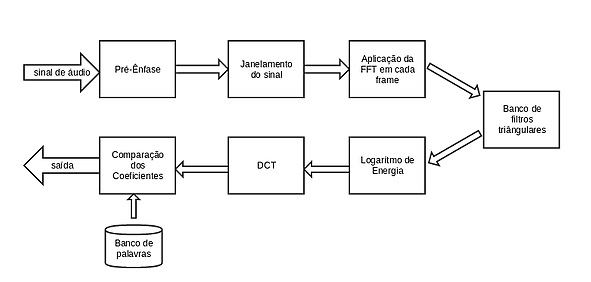
\includegraphics[width=10cm]{img/diaMFCC.jpg} % leia abaixo
\caption{Etapas para extração de coeficientes MFCC. \textit{fonte: Autoria própria}}
\label{fig:diaMFCC}
\end{figure}


O sinal de voz a ser parametrizado é passado através do filtro de pré-ênfase. Após o sinal ser filtrado, é necessário atenuar as descontinuidades causadas no início e no final de cada segmento, aplicando uma janela de Hamming de 25 ms de comprimento, com deslocamento de 10 ms, obtendo-se assim vetores MFCC a cada 10 ms. A terceira etapa consiste em aplicar a FFT para obter o espectro. Após a aplicação da FFT, aplica-se a equação \ref{eqima} para obter a potência espectral.

\begin{equation}
\label{eqima}
S[k] = |X[k]|^2 = (real(X[k]))^2 +  (imaginaria(X[k]))^2
\end{equation}


A próxima etapa consiste na aplicação do banco de filtros \textit{mel} à potência espectral. Os filtros \textit{mel} são definidos de acordo com a função \ref{filtro}.
\begin{equation}
\label{filtro}
%\begin{displaymath}
H_m[k] = \left\{\begin{array}{ll}
0 & k < k[m-1]\\
\displaystyle \frac{2(k-k[m-1])}{(k[m+1]-k[m-1])(k[m]-k[m-1])}, & k[m-1] \leq k \leq k[m] \\
\displaystyle \frac{2(k[m+1]-k)}{(k[m+1]-k[m-1])(k[m+1]-k[m])}, & k[m] \leq k \leq k[m+1] \\
0 & k > k[m+1]\end{array} \right.
%\end{displaymath}
\end{equation}

A Figura \ref{fig:filtro} mostra o banco de filtros usados na técnica MFCC. Cada filtro calcula a média do espectro em torno de um espectro central. Quanto maior a frequência, maior é a largura da banda.

\begin{figure}[H]
\centering % para centralizarmos a figura
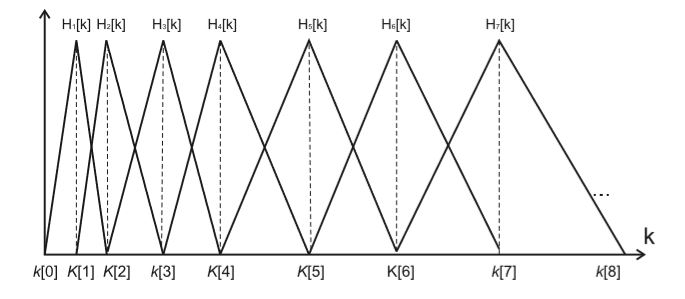
\includegraphics[width=10cm]{img/filtrotriangular.jpg} % leia abaixo
\caption{Banco de filtros triângulares MFCC. \textit{fonte: \cite{pucpncc}}}
\label{fig:filtro}
\end{figure}

Para determinar matematicamente os segmentos, parte- se da frequência extremas $f_l$ e $f_h$ que são as frequências de corte do banco de filtros em Hz. Esses valores são usados para dividir o intervalo em $B+1$ partes iguais. Para obter os valores em Hz, basta aplicar a função inversa \ref{inversa}.

\begin{equation}
\label{inversa}
k[m] = \big( \frac{N}{F_s}\big) Mel^{-1} \big(Mel(f_l) + m \frac{Mel(f_h)- Mel(f_l)}{M+1}\big)
\end{equation}

onde $F_s$ é a frequência de amostragem em Hz, M é o número de filtros e N o número de amostras da FFT. $k[m]$ são as frequências digitais e $Mel^{-1}$ determina a largura do banco de filtros e é dado por
\begin{equation}
Mel^{-1}(m) = 700(e^{\frac{m}{1125}} - 1)
\end{equation}

Em seguida, obtém-se a log-energia da saída de cada um dos filtros \textit{mel}. Por fim os coeficientes MFCC são obtidos aplicando a DCT ao logaritmo dos coeficientes de energia obtidos no passo anterior.



























